%# -*- coding:utf-8 -*-
\chapter{基于CTA的主动脉的分割与可视化}
\label{chap3} \fontsize{12pt}{12pt}\selectfont

\section{引言}

正如本文开篇所述,心血管疾病是一类对人类健康构成严重危害的疾病。
为了对这类疾病进行精确的诊断和治疗,研究人员已经成功研究了许多成像技术(见第\ref{sec2-2}节)。
血管系统本身特有的复杂的空间结构和多变的形态,决定了血管影像的大信息量、复杂特征。
于是,对血管影像的分割就成了一个通往血管模型的精确可视化的关键步骤。
在此基础上,医生才能对病情进行准确的诊断和治疗。
目前,尽管研究人员开展了大量关于血管分割的研究工作——有的已取得不俗成果,有的仍在进行;但是,血管分割仍然是一项极富挑战性的任务\cite{Lesage2009Review}。
没有一种分割方法能够独自解决当前所有影像模态获取的影像的分割问题。
分割完成后就要对分割所得信息进行图形处理,从而显示血管系统的几何外形。
我们采用行进立方体(Marching Cubes)方法\cite{Lorensen1987MC}将血管外表面所对应的像素值决定的空间曲面提取出来。
为了后续工作的需要,我们采用XXX方法计算血管模型的中心线;
利用XXX方法精简构成血管模型的多边形的数量;
利用XXX方法对多边形数量精简后的血管模型进行多边形三角化;
利用XXX方法对三角化后的血管模型进行几何外观上的平滑处理。

本章的叙述将按照研究工作的顺序依次展开。
首先,介绍基于CTA的血管系统的分割,描述工作中先后采用的两种不同分割技术的原理与实现,以及各自在算法层面的性能,并简要说明这两种技术各自的优势和劣势。
其次,介绍血管模型的可视化,描述工作中采用的主要技术方法的原理与实现。
再次,展示血管建模的实验结果。
最后,给出这部分工作的阶段性结论。

\section{基于CTA的血管系统的分割}

血管分割是一项难度较大的任务,其难度在于\cite{Lesage2009Review}:
一是影像采集过程中对信息造成的损害,如:对比度、解析度、噪声等;
二是血管系统本身的复杂结构,空间分布复杂、粗细和弯曲程度不一;
三是血管内部的支架、钙化物、血管瘤、管腔狭窄等能对血管系统的外观和几何结构产生影响;
四是血管系统深植于人体复杂的解剖环境当中,彼邻其他器官。
此外,由于血管影像的上述特点,使得血管影像的数据量很大、血管的图像特征很复杂,这都给图像分割算法的运算性能提出了更高的要求。

血管分割技术被广泛应用于脑、心、肺、肝、肾、以及肢体外周等部位的血管系统的分析与诊断。
获取血管影像的医学影像模态包括磁共振和CT等。
根据分割结果的不同,血管分割可分为血管腔分割、血管外壁分割、以及血管内血栓分割\cite{Lesage2009Review}。
由于血管成像时,对比剂的增强效果只能使血管内腔在影像中得以保留,故血管腔分割相对容易;而血管外壁和管内血栓的分割则相对较难。
在本文中,我们仅讨论与经皮冠状动脉导管介入术相关的血管系统的分割,影像模态为CT,影像中包含了病例人体的躯干,扫描时对血管系统进行了增强。
因为我们仅仿真血管内部的情况,所以只需进行血管腔的分割。

用于血管分割的方法多种多样,根据其基本的提取策略可以将这些方法分为区域生长法、活动围线法、以及基于中心线的方法。

\subsection{区域生长方法}

区域生长法是一类基于区域的图像分割方法,它的运行从最初给定的“种子区域”开始,根据使用者预先定义的“生长准则”把符合要求的像素或者子区域合并成为较大区域。
其中,“种子区域”通常是一个或多个像素(二维情形)或者体素(三维情形)。
“生长准则”则是根据处理任务而制定的,其主要限定特征是像素(或者体素)的灰度值或颜色\cite{Gonzalez2004Matlab}。
区域生长法所得结果就是使用者“感兴趣的图像区域”,使用这种方法进行分割的目的就在于此,这一目的能否达成,依赖于“种子”的选取和“生长准则”的制定。
表征区域生长法区别的主要特征有:“生长准则”、确定邻接像素的邻域连接类型、以及寻找邻接像素的策略\cite{Ibanez2005ITKGuide}。
区域生长法主要用于图像分割、以及图像的预处理等场合。

理想情况下,区域生长法的操作始于种子点的选取。
然后,我们将这些种子点分为$n$组(对应于分割目标中的$n$个物体),$A_1, A_2, \ldots, A_n$。
各分组中的种子点的个数可以为$1$,即该组中仅含有一个种子点,分组总数也可以为$1$,即分割目标只有一个。
接着,区域生长法在此基础上会求出一个对作用图像的曲面细分(Tessellation),这个细分将原图像划分为若干区域。
这些区域都具有这样的性质,即一个区域中,每个连接到的分量都与某一组种子点$A_i$相连。
受此约束,所选的区域都尽可能是“齐次的”\cite{Adams1994SRG}。

算法的每一步都在演进,借以向上述的种子点的集合中的其中一个添加一个像素。
现在,我们考虑该算法运行$m$步后,集合$A_i$的状态。
如果我们用$T$来表示所有与上述区域邻接而尚未被重新分配的像素的状态,那么
\begin{equation}
\label{eq3-1}
T = \left\{x\notin\bigcup_{i=1}^{n}A_i|N(x)\cap\bigcup_{i=1}^{n}A_i\neq\varnothing\right\}
\end{equation}
其中,$N(x)$是像素$x$邻接区域中像素所组成的集合。
下面,我们假定所讨论的算法作用于平面图像上,一个像素与其周围的像素的邻接形式是$8$-邻域。
若$\forall x\in T$,
则以$i(x)\in \left\{1, 2, \ldots, n\right\}$为上述某种子点集合$A$的下标,该集合满足$N(x)\cap\bigcup_{i=1}^{n}A_i\neq\varnothing$。
以$\delta(x)$表示$x$与其邻接区域的不同程度。
该$\delta(x)$可表示为
\begin{equation}
\label{eq3-2}
\delta(x)=\left|g(x)-\underset{y\in A_{i(x)}}{mean}[g(y)]\right|
\end{equation}
其中,$g(x)$是图像在像素$x$处的灰度值。
若$N(x)$与两个或更多的$A_i$集合相交,那么我们就将$i(x)$作为$i$的值,使得$N(x)$与$A_i$相交,且$\delta(x)$最小。
或者,在同样情况下,我们可能需要将$x$归为一个边界像素,并将之添加到集合$B$中,该集合包含了那些已经被发现的边界像素。
标定这些边界像素对满足显示需要或者下文提到的半交互修正流程都很有用。
我们取$z\in T$,使得
\begin{equation}
\label{eq3-3}
\delta(z)=\min\limits_{x\in T}{\left\{\delta(x)\right\}}
\end{equation}
并将$z$添加到$A_i(z)$中。

至此,算法就完成了第$m+1$步。
整个算法将依照上面介绍的过程重复运行,直到所有的像素都被恰当地分配为止。
此过程开始于每个种子点的集合$A_i$互不相交。
式\ref{eq3-2}和式\ref{eq3-3}所给出的定义保证在考虑连接性的约束的前提下,最终的分割结果由尽可能“齐次的”区域组成。

在区域生长法的程序设计中,我们采用了串列顺序列表(Sequential Sorted List, SSL),也就是计算机算法理论中的链表(Linked List)。
在区域生长法的情景下,SSL其实就是分割过程中,原始图像中的像素被读入内存后的地址,这些像素地址根据某种属性进行排列。
当在区域生长法的每一步开始时,我们从SSL的起始处取要考虑的下一个新像素。
当一个像素要被添加至SSL的时候,我们必须根据其自身具有的排序属性来选定这个像素在SSL中的位置。
在我们讨论的这种情况中,SSL根据$\delta$来收储集合$T$中的数据。

实现上述算法(边界标定的情形)的伪代码如下:
{\renewcommand{\baselinestretch}{1}{
\begin{algorithm}[htb]                    %算法的开始
\caption{\textsc{Seeded Region Growing}}  %算法的标题
\label{alg:SRG}                           %给算法一个标签,这样方便在文中对算法的引用
\begin{algorithmic}[1]   %不知[1]是干嘛的?
%\REQUIRE ~~\\            %算法的输入参数:Initialization
%  Set $J=0$; $S_0  = \left\{ \phi  \right\}$; $R(S_0 ) = 0$; $\Omega=\{1,2,\ldots,K\}$;
\ENSURE ~~\\             %算法的迭代:Iteration
%Ensemble of classifiers on the current batch,  $E_n$;
%\WHILE    {$J<M$}
%\STATE $J\leftarrow J+1$;
%    \FORALL {$k\in \Omega$}
%    \STATE  $R_{temp}=0$;  $\Delta R_{J,k} = R(S_{J-1}\cup \{k\})-R(S_{J-1})$;
%         \IF  {$\Delta R_{J,k}>0$}
%            \IF{$R(S_{J-1}\cup \{k\})\geq R_{temp}$}
%            \STATE $R_{temp}\leftarrow R(S_{J-1}\cup \{k\})$; $s_J\leftarrow k$;
%            \ENDIF
%         \ELSE
%            \IF{$1/(1-\Delta R_{J,k}/c_k )<rand(1)$}
%            \STATE $\Omega= \Omega-\{k\}$;
%            \ENDIF
%         \ENDIF
%    \ENDFOR
%\IF {$R_{temp}>0$}
%\STATE $S_J\leftarrow S_{J-1}\cup \{s_J\}$;
%\ELSE
%\STATE $J\leftarrow J-1$; Break;
%\ENDIF
%\ENDWHILE              %算法的返回值

\STATE Label seed points according their initial grouping.
\STATE Put neighbors of seed points (the initial T \ref{eq3-1}) in the SSL.
\WHILE {$SSL\neq \varnothing$}
    \STATE Remove first point $y$ from SSL.
    \STATE Test the neighbors of this point:
    \IF {all neighbors of $y$ which are already labeled (other than with the boundary label) have the same label}
        \STATE Set $y$ to this label.
        \STATE Update running mean of corresponding region.
        \STATE Add neighbors of $y$ which are neither already set nor already in the SSL to the SSL according to their value of $\delta$.
    \ELSE
        \STATE Flag $y$ with boundary label.
    \ENDIF
\ENDWHILE
%\LASTCON ~~\\          %OUTPUT
%  selected user set $S_J$ and weighted sum rate $R(S_J)$;

\end{algorithmic}
\end{algorithm}
}}

区域生长法充分图像的局部空间信息,它能有效地克服利用其他方法进行分割时,所得结果中有可能存在的图像空间不连续的问题。
然而,作为一种低层的图像分割方法,区域生长法也存在着一些不足。
首先,区域生长法在克服了前述问题的同时,容易造成过度分割(使分割结果中包含了一些使用者“并不感兴趣的区域”);
其次,区域生长法依赖人工交互以获得使处理得以进行的“种子”——这是由其基本特征所决定;
最后,区域生长法对图像中的噪声比较敏感,因此在引入这类方法之前,必需对被处理图像进行降噪处理。
除此之外,由于区域生长法属于串行算法,当欲分割目标较大时,处理速度就会明显变慢。
因此,在诊断场合中,此类方法一般用于对肿瘤和伤疤等目标进行分割。

\subsection{快速步进方法}

In this section the overall processing pipeline is discussed and the techniques used for the lumen segmentation of the abdominal aorta from CTA are detailed.
% The original data adopted in our work is a series of CTA images with the dimension of $512\times512\times90$.
% The series are acquired from the trunk of the patient with CVDs.

The overall design of the pipeline is illustrated in Fig. \ref{fig:DataFlow}.
The format and data type of original images are firstly converted.
Then the conditioned data is fed into two branches to produce the two inputs required by the main segmentation module.
One branch performs several preprocessing work on the images to produce the feature images. %, including smoothing, gradient magnitude computation, and intensity mapping.
And the other branch computes the initial level sets of the images. %, including a mini level set branch which requires numbers of seeds.
After the branches end the computation, their production are fed into the main segmentation module, where the actual interface evolution takes place.
In the final phase, the output level sets are extracted and then visualized by using a surface rendering technique.
%The parameters and seeds are provided manually and tuned repeatedly during the processing.
\begin{figure}[tb]
\centering
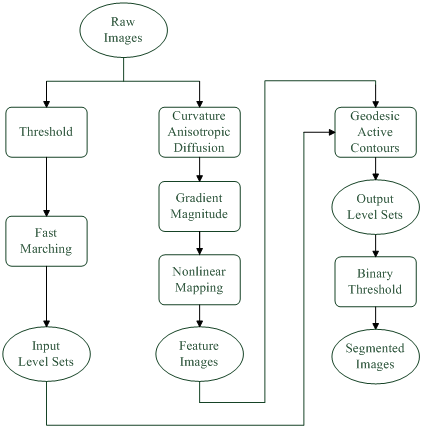
\includegraphics[width=3.2in]{Figures/DataFlow.png}
\caption{An overview of the segmentation pipeline.}
\label{fig:DataFlow}
\end{figure}

\subsection{Preprocessing}

Before the main processing begins, several necessary pretreatment on the original images should be done.
By considering the requirements of the methods chosen for this job, the preprocessing should include the production of feature images, and the generation of input level sets.
The feature images provide the main level set method with the ``maps" about where to stop, while the input level sets give the main functioning module the initial contours from where the actual interface evolution begins.

\subsubsection{Production of Feature Images}

%The branch of feature image production is depicted in Fig. \ref{fig:DataFlow}.
Image smoothing is a necessary job due to the original series acquired from the medical modality are often mixed with some noisy pixels.
What to take care of is that the original edges of the target (i.e., aorta) should be preserved as completely as possible while removing the noises.
Bear this in mind, a level-set curvature method with variable conductance \cite{Whitaker2001} is chosen for the job.
This method is good at enhancing and preserving edges, and is robust to the edge contrast.
It can be described as the following \emph{modified curvature diffusion equation} (MCDE):
\begin{equation}
\label{eqn:MCDE}
I_t = |\nabla I| \nabla \cdot c(|\nabla I|) \frac{\nabla I}{|\nabla I|},
\end{equation}
where $I = I(x, y, 0)$ represents the input image, $I_t(\cdot) = I(x, y, t)$ represents the output image generated over time $t$, and $c$ is the conductance function given by
$c(|\nabla I|) = k^2/(k^2 + |\nabla I|^2)$ with $k$ a parameter which determines the contrast of boundaries that will have significant effects on the smoothing.

After that, the computation of gradient magnitude is performed on the resulting series to detect the edge of target.
Since the feature images to be produced are required by the downstream geodesic active contours module, the most important step in this series of tasks is the computation of the magnitude of gradient pixel-wisely for the images:
\begin{equation}
\label{eqn:Gaussian}
I_{grad} = \exp(-|(\nabla \ast G) \cdot I_t|),
\end{equation}
where $I_{grad}$ is magnitude of the gradient at some point in the image, and $\nabla \ast G$ means the first order derivative of a Gaussian operator.

The computed edge images are mapped through a nonlinear relation (usually represented in the form of an S-shaped function) in order to get the feature images:
\begin{equation}
\label{eqn:Sigmoid}
I_{\sigma} = (I_{max} - I_{min}) \cdot \frac{1}{1 + \exp\left(-\frac{I_{grad} - n}{m}\right)} + I_{min},
\end{equation}
where $I_{\sigma}$ denotes the intensity values of the output image, $I_{max}$ and $I_{min}$ represent the maximum and minimum of the output intensity values, respectively; $m$ is a constant that controls the width of the input intensity range, and $n$ is a constant that gives an intensity around which the range is centered.
The mapping results may vary due to different choices of the parameters for the individual modules in the pipeline.

\subsubsection{Semi-Automatic Generation of Input Level Sets}

%The initial level set generation branch is parallel to the above one, which is responsible for the computation of the values required by the main evolution as its input level sets (see Fig. \ref{fig:DataFlow}).
% This branch is a mini level set that takes numbers of seeding points (or seeds) before the computation begins.
The first pass is a thresholding procedure that will strip out most of the irrelevant details of the images.
After the thresholding is done, the fast marching algorithm \cite{Sethian1999} could focus its evolution on the target with the appropriately selected seeding points.
For the curve $\mathcal{C}$ evolving over time $t$
\begin{equation}
\label{eqn:Curves}
\mathcal{C}(t) = \{(x,y) | T(x,y) = t\},
\end{equation}
where $(x,y)$ represents some point in the image, and $T(x,y)$ is the time of arrival.
The algorithm solves the following Eikonal equation (which is in fact a stationary Hamilton-Jacobi equation)
\begin{equation}
1 = | \nabla T | F,
\end{equation}
where $F$ denotes the velocity in the normal direction at some point $(x,y)$.
$\mathcal{C}$ propagates inwards when $F < 0$; it propagates outwards when $F > 0$.
The results of this computation are the time-crossing map in which contains of a series of curve interfaces at different time of evolution.

\subsection{Geodesic Active Contours Evolution}

%The module that actually working towards the segmentation is illustrated in Fig. \ref{fig:DataFlow}.
At this point, the geodesic active contours module has its two inputs available: the feature images and the initial level sets.
The feature images provide the maps for the interface evolution initialized by the input level sets.
The classical ``snakes" or active contour models for boundary detection were proposed by Kass et al. \cite{Kass1988}.
The idea is to evolve a contour $\mathcal{C}$ such that the edge of the object can be detected.
This evolution is achieved by minimizing an energy functional whose (local) minimum can be found at the edge of the object.
% This energy functional of the contour $\mathcal{C}_0$ in the classical snakes approach is given by (the denotation is adopted from \cite{Caselles1997})
% \setlength{\arraycolsep}{0.0em}
% \begin{eqnarray}
% \label{eqn:Snakes}
% E(\mathcal{C})&{}={}&\alpha \int_0^1 |\mathcal{C}'(q)|^2 dq + \beta \int_0^1 |\mathcal{C}''(q)|^2 dq \nonumber \\
                  % &&{-}\:\lambda \int_0^1 |\nabla I ( \mathcal{C}(q) ) | dq,
% \end{eqnarray}
\setlength{\arraycolsep}{5pt}
% where $\mathcal{C}(q)$ denotes the parametrized planar curve $\mathcal{C}(q):[0,1]\rightarrow \mathrm{R}^2$, $I:[0,a]\times [0,b]\rightarrow \mathrm{R}^{+}$ represents an image on which the edge detection task is carried out, and $\alpha$, $\beta$, and $\lambda$ are all real positive constants.
% The first two components control the smoothness of the curves to be detected, and the last one propagates the curve outwards (or inwards) until it ``touches" boundaries of the objects in the given image.
% The classical problem is to find the curve $\mathcal{C}$ that minimizes the energy functional $E$, for the given constants $\alpha$, $\beta$, and $\lambda$.
However, the curve in this approach cannot deal with the change of its topology so that detecting more than one object in the image is impossible without additional procedures \cite{Caselles1997}.
Caselles \textit{et al.} \cite{Caselles1997} improved the classical ``snakes" by proposing the geodesic active contours method, which allows to detect both the internal and external boundaries of several objects simultaneously.
This method incorporates the concepts of geodesic computation and level set evolution.
The proposed model is a particular case of the classical model:
\begin{equation}
\label{eqn:ParticularSnakes}
E(\mathcal{C}) = \alpha \int_0^1 | \mathcal{C}'(q) |^2 dq - \lambda \int_0^1 | \nabla I_{s} ( \mathcal{C}(q) ) |dq,
\end{equation}
where $\mathcal{C}(\cdot)$ denotes the parametrized planar curve $\mathcal{C}(q):[0,1]\rightarrow \mathrm{R}^2$, $I_{s}:[0,a]\times [0,b]\rightarrow \mathrm{R}^{+}$ represents an image on which the edge detection task is carried out.

To minimize the functional defined by (\ref{eqn:ParticularSnakes}), the curve at the points of maxima $|\nabla I_{s}|$ must be located.
During this process, certain level of smoothness of the curve also needs to be kept.
In (\ref{eqn:ParticularSnakes}), $|\nabla I_{s}|$ can be substituted by $-g(|\nabla I_{s}|)$, where $g(\cdot): [0, \infty) \rightarrow \mathrm{R}^{+}$ is a monotonically decreasing function. %such that $\lim_{x \to \infty} g(x) = 0}$.
Hence, a general energy functional is obtained
\begin{equation}
\label{eqn:GeneralEnergy}
E(\mathcal{C}) = \alpha \int_0^1 | \mathcal{C}'(q) |^2 dq + \lambda \int_0^1 g( | \nabla I_{s} ( \mathcal{C}(q) ) | )^2 dq.
\end{equation}
The aim of the evolution is trying to obtain
\begin{equation}
\label{eqn:MinModel}
\min \int_0^1 g(|\nabla I_{s} ( \mathcal{C} (q) )|) |\mathcal{C}' (q)| dq.
\end{equation}
% Thus the problem has been shifted from the minimization of (\ref{eqn:ParticularSnakes}) to the geodesic computation.
In (\ref{eqn:GeneralEnergy}), $g(\cdot)$ is equivalent to the speed of the evolution of the curve.
And it is also dependent upon the geometry of the image content.
For the ideal edges of the objects to be detected, the choice of parameter $g(\cdot)$ is independent of their geodesic computation.
So the minimum given in (\ref{eqn:MinModel}) can be rewritten as:
\begin{equation}
\label{eqn:MinModel2}
\min \int_0^1 g(I_{\sigma}) |\mathcal{C}' (q)| dq.
\end{equation}
To obtain the minimum given in (\ref{eqn:MinModel2}), the following Euler-Lagrange associated with this model needs to be calculated
\begin{equation}
\label{eqn:EvolutionModel}
\frac{\partial \mathcal{C}(t)}{\partial t} = g(I_{\sigma}) \kappa \mathcal{N} - (\nabla g(I_{\sigma}) \cdot \mathcal{N}) \mathcal{N},
\end{equation}
where $\kappa$ is the curvature of $\mathcal{C}(t)$, $\mathcal{N}$ is the unit inward normal vector. %, and the right-hand side of the equation is the computation of Euler-Lagrange.
This equation presents the way $\mathcal{C}$ evolving towards the boundaries of the objects to be detected.
The initial curve is marked as $\mathcal{C}(0) = \mathcal{C}_0$, which evolves to a (local) minimum of (\ref{eqn:MinModel2}).

According to (\ref{eqn:EvolutionModel}), this evolution will stop when $\frac{\partial \mathcal{C}(t)}{\partial t} = 0$, meaning that the boundaries of the objects are detected.
Suppose that the curve $\mathcal{C}$ is a level-set of a function $u(\cdot):[0,a] \times [0,b] \rightarrow \mathrm{R}$.
Regarding (\ref{eqn:MinModel2}) and (\ref{eqn:EvolutionModel}), the former geodesic calculation is transformed to finding the steady state solution of the following equation:
\begin{equation}
\label{eqn:LevelSetModel}
\begin{split}
\frac{\partial u}{\partial t} & = |\nabla u| \textrm{div} \left(g(I_{\sigma}) \frac{\nabla u}{|\nabla u|}\right) \\
                              %& = g(I_{\sigma}) |\nabla u| \textrm{div} \left(\frac{\nabla u}{|\nabla u|}\right) + \nabla g(I_{\sigma}) \cdot \nabla u \\
                              & = g(I_{\sigma}) |\nabla u| \kappa + \nabla g(I_{\sigma}) \cdot \nabla u,
\end{split}
\end{equation}
where $\kappa = \textrm{div}\left(\frac{\nabla u}{|\nabla u|}\right)$.
The right-hand side of this equation is the Euler-Lagrange of (\ref{eqn:MinModel2}).
% Here in this equation, $u$ is the embedding function mentioned above that deforms according to $u_t = \beta |\nabla u|$, where $\beta$ is a function computed on the level sets.
% From the perspective of image segmentation, a positive real constant $c$ is introduced in order to detect the boundaries of a non-convex object using a convex initial curve
% \begin{equation}
% \label{eqn:ImprovedLevelSetModel}
% \begin{split}
% \frac{\partial u}{\partial t} & = g(I) |\nabla u| \textrm{div} \left(\frac{\nabla u}{|\nabla u|}\right) + c g(I) |\nabla u| \\
                              % & = g(I) ( \kappa + c ) |\nabla u|.
% \end{split}
% \end{equation}

In order to increase the ``attractive force" to the contour towards the edges and allow the detection of non-convex objects, the term $cg(I_{\sigma})|\nabla u|$ is added to (\ref{eqn:LevelSetModel}):
\begin{equation}
\label{eqn:Geodesic1}
\frac{\partial u}{\partial t} = |\nabla u| \textrm{div} \left(g(I_{\sigma}) \frac{\nabla u}{|\nabla u|}\right) + c g(I_{\sigma}) |\nabla u|,
\end{equation}
where $c$ is a constant and $c \in \mathrm{R}^+$.
Regarding (\ref{eqn:LevelSetModel}), the above equation can be rewritten as
\begin{equation}
\label{eqn:Geodesic2}
\frac{\partial u}{\partial t} = g( I_{\sigma} )( c + \kappa ) |\nabla u| + \nabla u \cdot \nabla g(I_{\sigma}).
\end{equation}
% which means that the level sets move according to
The above equation can be transformed to the following equation
\begin{equation}
\label{eqn:Geodesic3}
\frac{\partial \mathcal{C}}{\partial t} = g(I_{\sigma}) ( c + \kappa ) \mathcal{N} - ( \nabla g(I_{\sigma}) \cdot \mathcal{N} ) \mathcal{N}.
\end{equation}
The solution to this object detection problem is equivalent to the zero level-set of the steady state ($u_t = 0$) of (\ref{eqn:Geodesic1}).
%Comparing (\ref{eqn:EvolutionModel}) and (\ref{eqn:Geodesic3}), one can find an added term $c g(I_{\sigma}) \mathcal{N}$, which is corresponding to the
% For the ideal edges of the objects to be detected, the choice of parameter $g$ is independent of their geodesic computation.
% It is a very simple edge detector which is given by the following equation
% \begin{equation}
% \label{eqn:EdgeDetector}
% g = \frac{1}{1+\|\nabla \hat{I}\|^p},
% \end{equation}
% where $\hat{I}$ denotes a Gaussian-smoothed image of the original $I$ and $p$ is the exponential of $\hat{I}$.
% What we are interested in is the time when the curve interface corresponding to the edges of the target.
% After the evolution stopped, a binary thresholder is provoked to take a ``snapshot" of this interface.
% This resulting level set should be the edges of the objects to be detected.

\subsection{Surface Extraction}

To visualize the surface model, the surface information should be firstly extracted by the marching cubes method \cite{Lorensen1987MC}.
As the initial step of surface extraction, arrays of cubes are created from the input with each cube consisting of eight pixels (four from one slice and the other four from the next slice).
Then the index for each cube is calculated by comparing the eight intensity values to the specified isovalue corresponding to the surfaces of the objects.
By referring to the triangulated cases with the indexes, the intersection patterns of the objects and the cubes can be roughly determined.
Then the precise edge intersections are computed using linear interpolation with the intensity values at each vertex of the cubes.
After that, the unit normals to the surface at each vertex of these cubes are computed via central differences.
The resulting triangles are then sent to the graphics systems and displayed by standard rendering techniques.
% The isovalue representing the edge of the segmented target is selected.
% Then the 3-D model of the target can be reconstructed.
% That is the 3-D surface model of the lumen of the aorta.

\section{Experiments and Results}

\subsection{Experimental Setup}
Many experiments were carried out using different parameters for the validation of the approach to segment the aorta from CTA.
In our case, the CTA series in DICOM format had been converted to the form of XML first.
Then the converted data was fed into the feature image production branch and input level sets generation branch.
The resulting data from the two branches were sent to geodesic active contours module in order to generate the final results.
Finally, the marching cubes method is used to visualize the segmented data.
The experiments were all run on a machine with Intel's 2.83GHz Core 2 Quad CPU and 4GB RAM.

The input series was obtained by a 128-slice Siemens SOMATOM Definition Flash CT with the slice thickness of 0.6mm.
And the series contains the patient's entire abdominal aorta.
For illustrative purposes, a typical slice was selected from the series.
To reduce the computation time, the region that contains the major branches of the abdominal vasculature in the selected image were cropped (see Fig. \ref{fig_roi}).
\begin{figure}[tb]
\centering
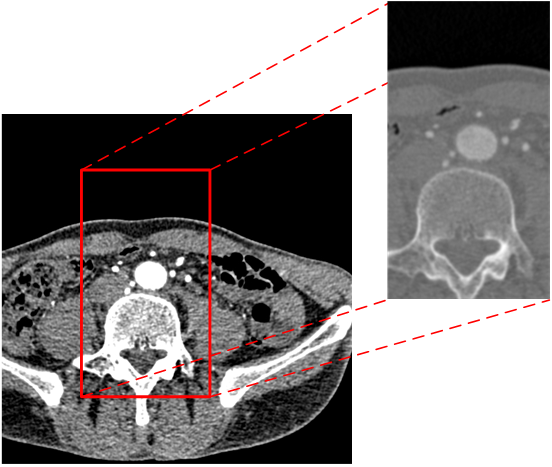
\includegraphics[width=2.5in]{Figures/ROI.png}
\caption{A typical ROI extraction of the original slice.}
\label{fig_roi}
\end{figure}
% Then the segmentation process was split into two branches first and then merged into the main evolution pipeline.
%This two-branching structure is built due to the two essential requirements of geodesic active contours module: the feature images and initial level sets.

\subsection{Feature Images}
In the feature image production branch, the following preprocessing tasks were performed sequentially:
\begin{enumerate}
\item removing noises without affecting the edges;
\item computing the gradient magnitude pixel-wisely;
\item mapping the intensity into the required feature.
\end{enumerate}
At the beginning, a level-set curvature method with variable conductance was utilized to perform the smoothing task.
It is an edge-preserving smoothing method that can remove the unnecessary noises from the images while preserving the nature of the boundaries of the objects.
The image was smoothed nicely and the boundaries of the aorta even the minor vessels (which means weaker edges) were preserved (see Fig. \ref{fig:Smoothing}).
Then the gradient magnitude module was introduced to fulfill the requirements of gradient computing.
It computes the magnitude of the gradient pixel-wisely for the image by performing the convolution with the first order derivatives of a Gaussian kernel defined by (\ref{eqn:Gaussian}).
%The only parameter of the kernel is its deviation $\sigma$ and we set it to 0.9.
The edges of the vessels, bones, and skins were extracted completely in the resulting image (see Fig. \ref{fig:Gradient}).
After computing the magnitude of the gradient, the non-linear intensity mapping was employed to generate the edge potential map.
The choices of the parameters in (\ref{eqn:Sigmoid}) heavily depends on extreme values of the pixel intensities in the gradient image.
In this case, to reverse the relationship between objects (in low intensities in the gradient map) and their edges (in high intensities in the gradient map), $m$ was set to be a negative value and $n$ to be a positive value which is larger than $|m|$.
The mapping produced the expected feature image with the proximities of the edges of the objects in zero intensity (see Fig. \ref{fig:Sigmoid}).
This made the evolution of the level sets driven by (\ref{eqn:Geodesic3}) propagated faster in the ``flat area" (with uniformly high intensities), whilst much slower (in a speed of about zero) in the ``ridge" (with rapid decreasing intensities).
\begin{figure*}[t]
\centering
%\subfloat[Smoothing with edge preserving (Conductance parameter = 0.9)]{\includegraphics[width=1.2in]{fig/dcm_smoothing.jpg}%
\subfloat{\includegraphics[width=1.2in]{Figures/dcm_smoothing.jpg}%
\label{fig:Smoothing}}
\hfil
%\subfloat[Computation of magnitude of gradient with Gaussian kernel ($\sigma = 0.9$)]{\includegraphics[width=1.2in]{fig/dcm_gradient.jpg}%
\subfloat{\includegraphics[width=1.2in]{Figures/dcm_gradient.jpg}%
\label{fig:Gradient}}
\hfil
%\subfloat[Nonlinear mapping using an S-shaped function ($m = -3$, $n = 20$)]{\includegraphics[width=1.2in]{fig/dcm_sigmoid.jpg}%
\subfloat{\includegraphics[width=1.2in]{Figures/dcm_sigmoid.jpg}%
\label{fig:Sigmoid}}
\caption{Producing the feature image in three steps: (a) smoothing with edge preserving ($\text{conductance parameter} = 0.9$); (b) computation of magnitude of gradient with Gaussian kernel ($\sigma = 0.9$); (c) nonlinear mapping using an S-shaped function ($m = -3$, $n = 20$).}
%\caption{Producing the feature image.}
\label{fig:PotentialImageGeneration}
\end{figure*}
\begin{figure*}[htb]
\centering
%\subfloat[Thresholding]{\includegraphics[width=1.2in]{fig/dcm_threshold.jpg}%
\subfloat{\includegraphics[width=1.2in]{Figures/dcm_threshold.jpg}%
\label{fig:Threholding}}
\hfil
%\subfloat[Level set evolution using fast marching method]{
\includegraphics[width=1.2in]{fig/dcm_fastMarching.jpg}%
\subfloat{
\includegraphics[width=1.2in]{Figures/dcm_fastMarching.jpg}%
\label{fig:FastMarching}}
\hfil
%\subfloat[Edge detection using geodesic active contours]{\includegraphics[width=1.2in]{fig/dcm_geodesic.jpg}%
\subfloat{\includegraphics[width=1.2in]{Figures/dcm_geodesic.jpg}%
\label{fig:GeodesicActiveContours}}
\hfil
%\subfloat[Binary thresholding]{\includegraphics[width=1.2in]{fig/dcm_out.jpg}%
\subfloat{\includegraphics[width=1.2in]{Figures/dcm_out.jpg}%
\label{fig:BinaryThresholding}}
\caption{Level set evolution: (a) thresholding ($\text{lower threshold} = 300\text{HU}$, $\text{higher threshold} = 2000\text{HU}$); (b) initial level set evolution from one seeding point using fast marching method; (c) edge detection using geodesic active contours; (d) binary thresholding to inverse the pixel intensities (intensity of the light area: $255$, intensity of the dark area: $0$).}
\label{fig:LevelSetEvolution}
\end{figure*}

\subsection{Level Sets Evolution}
The initial level set generation branch works for the level sets that required by the geodesic active contours module.
In this process, the thresholding module was called first to trim off the irrelevant organs with lower intensities, such as lungs, liver, kidneys, bowels, stomach, etc. (see Fig. \ref{fig:Threholding}).
%In our case, we set the lower and upper threshold values at 300HU (HU is short for Hounsfield Unit) and 2000HU, respectively.
This can further reduce the hunger for memory and dramatically shorten the computation time.
When finished this, the fast marching module is provoked to generate the initial interfaces.
One seed located interior of the region representing the aorta was fed to this module in this two dimensional image.
% And these seeds evolved the interfaces surrounding themselves respectively towards each other (see Fig. \ref{fig:FastMarching}).
And the time of arrival $T(x,y)$ given in (\ref{eqn:Curves}) were computed (see Fig. \ref{fig:FastMarching}).
Considering the prolonged geometric nature of the aorta and the characteristics of the algorithm, multiple seeding points inside the space representing the aorta should be fed in the three dimension case to acquire better results and much shorter computation time.
% We set the stopping time for the fast marching filter in order to shorten the time for the generation of initial level sets.

% \subsection{Geodesic Evolution}
The geodesic active contours evolution began working when all the preceding computation finished.
The module took the feature image and the initial contours as its inputs.
The contours evolved by the drive defined by (\ref{eqn:Geodesic3}) with the feature image as their reference.
The segmentation module evolved the contours until the edges were met (see Fig. \ref{fig:GeodesicActiveContours}).
After that, a binary thresholding step was performed to fill the inner area of the final contours as the light zone while the outer area as the dark zone.
This result is illustrated in Fig. \ref{fig:BinaryThresholding}.
All the parameters chosen manually to make the drive suitable to evolve the contour to the expected results were reused in the three dimensional case.

\subsection{Surface Construction Based on Segmentation Results}
Finally, the resulting volume were processed using the marching cubes method \cite{Lorensen1987MC}.
The isovalue corresponding to the edge of the lumen of abdominal aorta was picked manually.
Here the higher threshold value of the binary thresholder was provided as the isovalue for the isosurface extraction.
This ensured that the rendered surface representing the surfaces of the lumen of the aorta.
The final visualization model is depicted in Fig. \ref{fig:VisualizationModel}.
%From this figure, we can see that the lumen of the aorta was extracted successfully using the approach described here.
\begin{figure}[!htb]
\centering
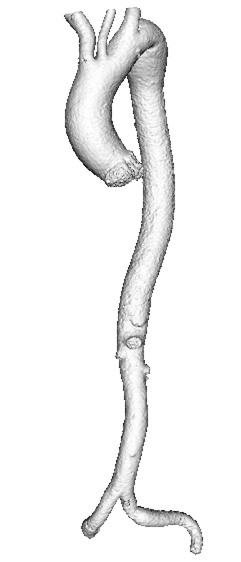
\includegraphics[width=1.1in]{Figures/model.png}
\caption{3-D surface model of the lumen of the aorta.}
\label{fig:VisualizationModel}
\end{figure}


\section{Conclusions and Future Work}
%The conclusion goes here.

The three dimensional model of the aorta is one of the most important parts of the virtual scenarios of the robotic training systems which is built for the intravascular surgical robot.
In this paper, a robust and semi-automatic vessel segmentation approach based on geodesic active contours method has been proposed.
After reporting the design and considerations of the experiments, the results as well as the analysis were presented.
The lumen model of the aorta was then reconstructed by the marching cubes method using the segmented volumetric data.
The experimental results showed that the approach can successfully deal with the messy part due to the anatomic nature of the adherence of the aorta and the spine; and can accurately gain the vessel model.

% The pipeline in this paper was programmed mostly in C++.
%Some of the imaging filters were implemented based on the Insight Toolkit (ITK) \cite{Ibanez2005ITKGuide}.
The data format of the original CTA series were firstly converted.
Then the converted data was fed into the pipeline and was transferred into two branches: one for the production of featured images, and the other for the production of initial level sets.
The production served as the input of geodesic active contours module.
%Moreover, we also provide series of parameters for this module thus it can start the interface evolution.
The evolution stopped after a specified number of iterations and the binary threshold module was called to converse the pixel intensity.
Then the marching cubes implementation extracted the surfaces of the aorta in the segmented data before rendering.

As a future work, on the one hand the coronary arteries needs to be segmented and visualized in the volumetric data.
On the other hand, a series of post-processing work will be carried out in order to eliminate the artifacts and decimate the number of polygons that consisting the surface model.
The whole vasculature model will be available to the simulation tests of the models of the catheters/guidewires.
%Besides, the improvement of the visualization effect of the vessel model will also be an substantial work.
%During this process, a friendly software interface of the surgical simulator will be implemented.


\section{本章小结} 